\documentclass{beamer}

% Theme
\usetheme{Madrid}

% Packages
\usepackage{tikz}
\usetikzlibrary{shapes.geometric, arrows.meta, positioning}

% TikZ Styles
\tikzset{
    block/.style={
        rectangle,
        rounded corners,
        draw=black,
        minimum width=3cm,
        minimum height=1cm,
        align=center
    },
    arrow/.style={
        thick,->,>=stealth
    }
}

% Title Info
\title{Food Surplus Redistribution System}
\subtitle{Connecting Restaurants with NGOs to Reduce Food Wastage}
\author{}
\date{}

\begin{document}

%----------------------------
\begin{frame}
\titlepage
\end{frame}

%----------------------------
\begin{frame}{Problem Statement}
\begin{itemize}
\item Large amounts of edible food are wasted daily.
\item NGOs face shortage of food resources.
\item No centralized digital system exists.
\item Manual coordination is inefficient.
\end{itemize}
\end{frame}

%----------------------------
\begin{frame}{Project Objectives}
\begin{itemize}
\item Reduce food wastage
\item Support NGOs
\item Enable real-time communication
\item Ensure transparency
\end{itemize}
\end{frame}

%----------------------------
\begin{frame}{Proposed System}
\begin{itemize}
\item Restaurants upload surplus food
\item NGOs view and request food
\item Restaurants approve requests
\item NGOs collect food
\end{itemize}
\end{frame}

%----------------------------
\begin{frame}{Major Modules}
\begin{itemize}
\item Restaurant Module
\item NGO Module
\item Admin Module
\item Notification Module
\item Database Module
\end{itemize}
\end{frame}

%----------------------------
\begin{frame}{Technology Stack}
\begin{itemize}
\item Frontend: HTML, CSS, JavaScript
\item Backend: Python (Flask/Django) or Java (Spring Boot)
\item Database: MySQL / MongoDB
\item Hosting: Cloud Platform
\end{itemize}
\end{frame}

%----------------------------
\begin{frame}{System Architecture Diagram}

\centering
\begin{tikzpicture}[node distance=3cm]

\node (restaurant) [block] {Restaurant};
\node (platform) [block, right=of restaurant] {Web / App Platform};
\node (ngo) [block, right=of platform] {NGO};
\node (database) [block, below=of platform] {Database};

\draw [arrow] (restaurant) -- (platform);
\draw [arrow] (platform) -- (ngo);
\draw [arrow] (platform) -- (database);
\draw [arrow] (database) -- (platform);

\end{tikzpicture}

\end{frame}

%----------------------------
\begin{frame}{System Flowchart}

\centering
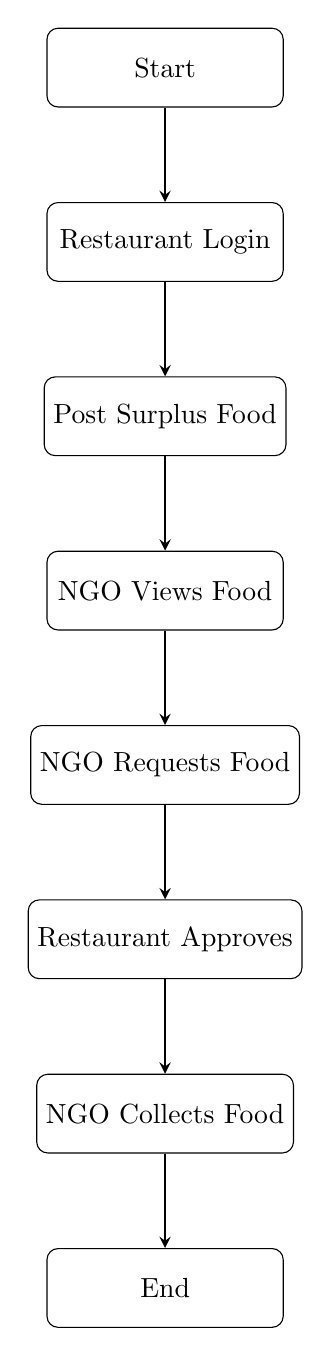
\begin{tikzpicture}[node distance=1.2cm]

\node (start) [block] {Start};
\node (login) [block, below=of start] {Restaurant Login};
\node (post) [block, below=of login] {Post Surplus Food};
\node (view) [block, below=of post] {NGO Views Food};
\node (request) [block, below=of view] {NGO Requests Food};
\node (approve) [block, below=of request] {Restaurant Approves};
\node (collect) [block, below=of approve] {NGO Collects Food};
\node (end) [block, below=of collect] {End};

\draw [arrow] (start) -- (login);
\draw [arrow] (login) -- (post);
\draw [arrow] (post) -- (view);
\draw [arrow] (view) -- (request);
\draw [arrow] (request) -- (approve);
\draw [arrow] (approve) -- (collect);
\draw [arrow] (collect) -- (end);

\end{tikzpicture}

\end{frame}

%----------------------------
\begin{frame}{Advantages}
\begin{itemize}
\item Reduces food wastage
\item Helps needy people
\item Easy to use
\item High social impact
\end{itemize}
\end{frame}

%----------------------------
\begin{frame}{Future Enhancements}
\begin{itemize}
\item Mobile Application
\item GPS-based pickup
\item AI-based prediction
\item Quality verification
\end{itemize}
\end{frame}

%----------------------------
\begin{frame}{Conclusion}
The system creates a digital bridge between restaurants and NGOs, reducing waste and supporting hunger relief.
\end{frame}

\end{document}
